\documentclass[12pt]{article}
\usepackage{geometry}
\usepackage{float}
\usepackage{hyperref}

\usepackage[sfdefault]{inter}
\usepackage[scaled=0.8]{cascadia-code}
\usepackage{setspace}

\usepackage{caption}
\captionsetup{%
   labelfont=bf,
   format = plain,
   font = footnotesize
}

\usepackage{biblatex}
\addbibresource{bibliography.bib}

\usepackage{titlesec}

\titleformat*{\section}{\LARGE\bfseries}
\titleformat*{\subsection}{\large}
\titleformat*{\subsubsection}{\large}
\titleformat*{\paragraph}{\large}
\titleformat*{\subparagraph}{\large}

\renewcommand*\contentsname{Resumen de los contenidos}
\renewcommand{\listfigurename}{Tabla de Figuras}

\hyphenpenalty=10000

% Comand para keywords
\providecommand{\keywords}[1]
{
  \small	
  \textbf{\textit{Keywords---}} #1
}

% Setup de hiperenlaces
\hypersetup{
    colorlinks=true,
    linkcolor=cyan,
    filecolor=magenta,      
    urlcolor=cyan,
    pdftitle={_deadSet},
    pdfpagemode=FullScreen,
}
 \geometry{
 a4paper,
 total={170mm,257mm},
 left=20mm,
 top=20mm,
 }
 \usepackage{graphicx}
 \usepackage{titling}

 \title{\textbf{\Huge{Videojuego creado en Unity:\\
 \vspace{5mm}
 \textunderscore deadSet
  }
 }
}
\author{\large{Jesús Jiménez Montero}}
\date{Diciembre 2022}
 
 \usepackage{fancyhdr}
\fancypagestyle{plain}{%  the preset of fancyhdr 
    \fancyhf{} % clear all header and footer fields
    \fancyfoot[R]{
\includegraphics[width=2cm]{Images/uanl (1).jpg}}
    \fancyfoot[L]{\thedate}
    \fancyhead[L]{Videojuego creado en Unity: \textunderscore deadSet}
    \fancyhead[R]{\theauthor}
}
\makeatletter
\def\@maketitle{%
  \newpage
  \null
  \vskip 1em%
  \begin{center}%
  \let \footnote \thanks
    {\LARGE \@title \par}%
    \vskip 1em%
    %{\large \@date}%
  \end{center}%
  \par
  \vskip 1em}
\makeatother

%___________________________________________________________
%___________________________________________________________
%___________________________________________________________
%___________________________________________________________
%___________________________________________________________

\begin{document}
\graphicspath{ {./images/} }
%___________________________________________________________

\vspace{5cm}
\maketitle

\vspace{2cm}

\begin{figure}[H]
    \centering
    
\includegraphics[scale = 1.5]{Images/uanl (1).jpg}
\end{figure}

\vspace{2cm}

\begin{center}
    \begin{tabular}{@{}ll}
        
        \vspace{1cm}
        \theauthor\\
        \vspace{1cm}
        \large{VJ1202: Informática Básica}\\
        \vspace{1cm}
        \large{Raúl Montoliu Colás}
    
    \end{tabular}
\end{center}

%___________________________________________________________
%___________________________________________________________
%___________________________________________________________
%___________________________________________________________

\spacing{1.5}

\newpage
\begin{abstract}
    \textunderscore deadSet es un videojuego de acción, estilo twin-stick shooter \cite{twinstickshooters} \footnote{\textit{De Wikipedia: shooter multidireccional en el que el personaje del jugador se controla con dos joysticks: uno para moverse y otro para apuntar y disparar a los enemigos.}} 
    con aspecto roguelike \cite{roguelike}. La misión del jugador es sobrevivir el máximo tiempo posible a oleadas de zombis, hasta que llegue la ayuda (la cual nunca llega). Además, de tener dos armas, un rifle y una escopeta, la cual recarga la munición del rifle. El proyecto consta de la creación de un videojuego creado en Unity, siguiendo las pautas marcadas con el tutorial de Unity dado en clase: “Ruby’s Aventure”. 

    _deadSet
    \keywords{Videojuego, Unity, Roguelike}
\end{abstract}
\newpage

\tableofcontents
\newpage

\listoffigures
\newpage

%___________________________________________________________
%___________________________________________________________
%___________________________________________________________
%___________________________________________________________

\section{Propuesta de juego}

    Este juego nació como una idea basada en otro juego, aunque lamentablemente requería demasiado tiempo y conocimiento de los cuales no se disponía, por lo que se simplificaron muchas ideas, llevando a \textunderscore deadSet. 

    Se quería desarrollar un juego que fuese como la frase en inglés indica: \textit{"easy to learn, hard to master"} \footnote{\textit{Fácil de aprender, díficil de dominar}}; pero que fuese lo más rejugable posible. Por lo tanto, se eligió el género de juegos roguelike para esta labor. 

%___________________________________________________________
%___________________________________________________________
%___________________________________________________________
%___________________________________________________________

\section{ Herramientas usadas en el proyecto}

    Se utilizaron numerosas herramientas para la realización de este juego, las cuales se agruparan por el uso dado:

    \subsection{Programación}
        \begin{itemize}
            \item Unity 2020.3.42/43 LTS: Motor de juegos.
            \item Rider 2022.3: IDE con una integración muy elevada con Unity. 
            \item Github (desktop): Gestor .git para gestionar copias del código.
        \end{itemize}
        
    \subsection{Arte}
        \begin{itemize}
            \item Aseprite: Editor de imágenes especializado para pixel-art. 
        \end{itemize}

    \subsection{Redacción de documentos}
        \begin{itemize}
            \item Overleaf: Procesador de documentos basado en el lenguaje LaTeX. 
        \end{itemize}


%____________________________________________________________________________________
%____________________________________________________________________________________
%____________________________________________________________________________________
\section{Puntos clave del juego y target}
    Los puntos clave de \textunderscore deadSet se pueden resumir de esta manera: 
    \begin{itemize}
        \item Sistema de combate simple, pero complicado de dominar que balancea el \textit{flow} del juego.
        \item La rejugabilidad es un aspecto importante del juego, haciendo que el jugador quiera mejorar sus tiempos cada vez que quiera jugar. 
        \item Debido a sus gráficos simples realizados en \textit{pixel-art}, el juego se podrá jugar en una gran cantidad de ordenadores. 
        \item Aunque el juego dispone de mucha rejugabilidad, se pretende ser respetuoso con el tiempo del jugador, con las partidas durando de media entre 5 a 10 minutos, siendo más si el jugador obtiene mucha habilidad. 
    \end{itemize}
        
        \subsection{Taxonomía de Bartle}
            Otro aspecto crucial del juego es su \textit{target} es muy definido. Para lograr esto, se usó la \textit{Taxonomía de jugadores de Bartle}, la cual se define como: 
                \begin{itemize}
                    \item \textit{\textbf{Achievers}}: Los cuales prefieren, por ejemplo,  ganar la máxima puntuación en un juego o conseguir todos los logros en un juego. 
                    \item \textit{\textbf{Killers}}: que son los jugadores que prefieren interactuar con otros jugadores y superarlos en algún reto.
                    \item \textit{\textbf{Explorers}}: Que, si tienen un mapa el cual revela el mundo de forma progresiva, preferiran completar el mapa entero y descubrir todos los recovecos que este mundo esconda.
                    \item \textit{\textbf{Socializers}}: Que están dispuestos a relacionarse con la mayor cantidad de jugadores posibles y prefieren el aspecto social de juego. 
                \end{itemize}
    
            \vspace{5mm}
    
            Una vez definida la \textit{Taxonomía de Bartle} podemos definir los jugadores que más llamará la atención para jugar \textunderscore deadSet serían: 
                \begin{itemize}
                    \item \textit{\textbf{Killers}}: Debido a que el juego se basa principalmente en superar oleadas de enemigos los cuales hay que derrotar usando armas.
                    \item \textit{\textbf{Achievers}}: Debido a la presencia de un temporizador dentro del juego que hará que este tipo de jugadores que quiera superar cada vez que juegen.
                \end{itemize}

%____________________________________________________________________________________
%____________________________________________________________________________________
%____________________________________________________________________________________

\section{Jugabilidad y Mecánicas}
    \subsection{Modo de juego}
        El juego dispone de un único modo de juego, el cual es el modo de oleadas de enemigos, en el que el jugador se enfrenta a enemigos generados aleatoriamente por el mapa y una vez son derrotados, el juego genera más enemigos dependiendo del número de oleadas.

    \subsection{Dinámicas}
        La dinámica más presente del juego es la gestión de munición, ya que el jugador tiene que tener en mente el número de balas restantes; además de que todas las acciones del jugador requieren de un tiempo para realizarse, siendo una de las más duras recargar la escopeta porque se necesita munición de escopeta para recargar el rifle. 
    
    \subsection{Mecánicas de combate}
        \textunderscore deadSet es un roguelike en el que si el jugador muere, la partida se acaba y el juego se reiniciará desde la oleada 1. El jugador, para defenserse de los zombies, se le proporciona dos armas:
        
            \begin{itemize}
            
                \item \textbf{Rifle de asalto}: Rifle con una alta cadencia de tiro y preciso pero un daño bajo. Versátil y es capaz de derrotar varios enemigos con un cargador, aunque, no se puede recargar de forma manual.\\ Como mecánica adicional, el jugador recarga el rifle disparando la escopeta; es decir, cuando el jugador dispara la escopeta, se restaura el cargador del rifle.
                
                \item \textbf{Escopeta}: Arma muy potente, capaz de derrotar un enemigo de un solo disparo; aunque lenta de usar. Es el arma primaria del jugador debido a que es muy potente, aunque al contrario del rifle, se necesita recargar la escopeta de forma manual usando un botón.\\ 
                Por motivos de balanceo, el cargador de la escopeta es pequeño y se recarga como una escopeta de bombeo (es decir, cada vez que el jugador dispara tiene que esperar para disparar de nuevo), además de para recargarla se hace cartucho a cartucho (es decir, se introduce una bala en el cargador cada cierto tiempo).
            \end{itemize}

        
        Además, cada oleada acabada en 1, activa un método (ver código debajo) para mejorar las armas las cuales mejoran de forma ligera las estadísticas hasta llegar a un umbral concreto.
        
    \begin{verbatim}
    if (waveNumber % 10 == 1 && waveNumber != 1)
    {
        UpdateWeapons();
    }
    \end{verbatim}

    Otros aspectos destacables del combate es cuando se daña el personaje o los zombies. Comenzando por los zombies: 
    
    cuando una bala lo toca, cambia su color para señalizar que ha sido golpeado, y suavmente vuelve a su color original; esto se hizo para darle más importancia al golpe y resaltar al jugador que ha dañado al enemigo. 

    Esto también ocurre cuando los zombis dañan al jugador. El zombi que ha golkpeado al jugador se resalta (esta vez la duración siendo el \textit{cooldown} necesario para volver a hacer daño al jugador). 
    
    Esto también ocurre con el sprite del jugador para resaltar que ha sido dañado. El desvanecimiento del color es el mismo que el \textit{cooldown} de los zombis y puede ser activado tantas veces el jugador se choque contra un zombi.

        \subsection{Bucle de juego}
        \textunderscore deadSet se caracteriza por tener un bucle de juego muy definido y cerrado, el cual se puede definir como:
        
        \begin{itemize}
            \item Derrotar oleada de enemigos → Pasar de oleada → Oleada Fuerte → Mejora de Armas → Repetir
        \end{itemize}
        Este de hecho se podría definir como el bucle de juego principal, aunque hay otros bucles aún más cerrados, pero menos obvios al jugador debido a que se integran con este. 
        
        Estos bucles serían, por ejemplo, el propio hecho de usar las armas. Aunque tampoco se puede considerar un bucle cerrado, ya que las armas se pueden usar en el orden que el jugador quiera. Podemos representarlo como un bucle de ejemplo: 
        \begin{itemize}
            \item Disparar rifle → Agotar munición → Disparar escopeta → Disparar rifle → Agotar ambas municiones → Recargar escopeta → Repetir
        \end{itemize}
%____________________________________________________________________________________
%____________________________________________________________________________________
%____________________________________________________________________________________
\section{Elementos que componen el juego}
    En este aparatado se explican los assets que componen el juego, los cuales están listados de forma concisa en el \href{https://github.com/JesusJMUJI/TopDownShooterGame}{GitHub del proyecto}. 
    
    \subsection{Interfaz de Usuario}
        Uno de los objetivos que se querría conseguir con el juego era ser minimalista en cuanto al diseño, incluyendo la interfaz.  
        \begin{figure}[H]
            \centering
            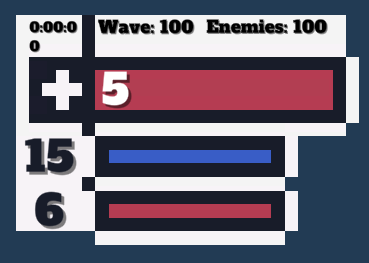
\includegraphics[scale = 0.7]{Images/UI.png}
            \caption{Interfaz del juego}
            \label{fig:UI}
        \end{figure}
        
        Se usaron elementos minimalistas para generar la interfaz del juego, con un aspecto de bloques y números con fuente lo más legible posible. Con las barras de munición (azul y rojo para el rifle y la escopeta, respectivamente) agotándose según las balas restantes en el cargador, además del número mencionado para los que jugadores que prefieran saber exactamente cuanta munición les queda.
        
        Se probó otra variante de los contadores, incluyéndolos al lado del arma. Aunque se descartó la idea debido a que los contadores eran demasiado pequeños y podían dar lugar a confusión al leerlos.
        
        \begin{figure}[H]
            \centering
            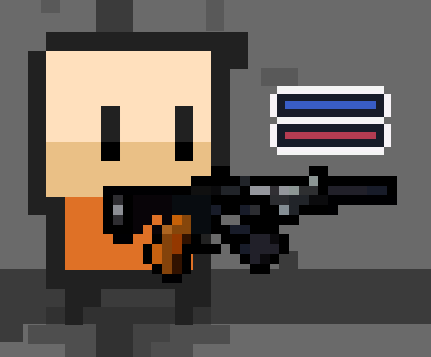
\includegraphics[scale = 0.5]{Images/UI descartada.png}
            \caption{Interfaz al lado del arma}
            \label{fig:UI descartada}
        \end{figure}
        
    \subsection{Elementos gráficos}
        
        Para simplificar el proceso de desarrollo del juego, se utilizaron assets comprados con licencia de uso personal/comercial, los cuales se pueden encontrar en el \href{https://github.com/JesusJMUJI/TopDownShooterGame}{GitHub del proyecto}.
        
        Un resumen del uso de los assets gráficos sería:
        \begin{itemize}
            \item \textbf{2D Top Down Shooter Game Assets}: Starter Kit, para el \textit{tileset}, los personajes y la cruceta.
            \item \textbf{Tech Dungeon: Roguelite}, para interfaz del juego. (Demo del paquete)
            \item \textbf{Pixel Art Guns Pack + Animations}: Para las armas con sus respectivas animaciones, además de las balas.
        \end{itemize}
        
        Aun habiendo usado assets comprados, se quiso dar un toque personal al juego, creando el logotipo a mano. Para esta labor, se usó el software gráfico Aseprite, dando este resultado:
        \begin{figure}[H]
            \centering
            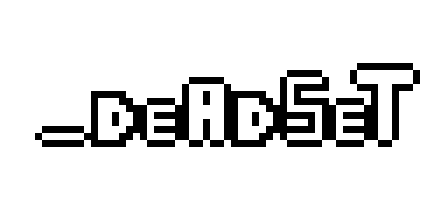
\includegraphics[scale = 0.5]{Images/logo_big.png}
            \caption{Logotipo del juego}
            
        \end{figure}
        
        Para futuros proyectos, un objetivo a alcanzar sería poder realizar todos los assets gráficos a mano.
    
    \subsection{Apartado sonoro}
        
        Para el sonido del juego, se tenía un objetivo en mente, el cual es: \textit{“punchy”}, traducido al castellano como “impactante”. Se buscaban sonidos que fuesen poco monótonos, ya que el juego se basa en disparar todo el tiempo, así que no se podían usar sonidos que fuesen genéricos o “aburridos”. 

        Además, un problema que el jugador que presentarse es, quedarse sin munición. Se quería que el jugador siempre tuviese presente su número de balas restante y para indicar que su cargador se había agotado, se añadió un \textit{click} cuando intentas disparar y no te queda munición. 
        
        Se usaron los sonidos del paquete \textit{Snake's Authentic Gun Sounds(1 y 2)}.
        
        Aparte de los sonidos de \textit{Snake}, se usó para sonido de la esscopeta un sonido de una librería C00: Sonniss.com - GDC 2016 - Game Audio Bundle / TS Sound → 12 Gauge Shotgun.
        
        Para la música se necesitaba música que no hiciese monótona las partidas, ya que, un juego que esté diseñado para ser regulable necesita precisamente romper esta, un ejemplo para resolver esto es que cada vez una canción acaba, se escoge de forma aleatoria una canción de una lista de canciones. 
        
        Para estas canciones se usó la música de \textit{Action Music Pack 1 y 2}.
        
    \subsection{Otros elementos}
    
        Comentando otros assets usados en el juego, para el menú principal se usaron sprites del paquete: \textit{Controller \& Keyboard Icons}, ya que se quería representar los controles una manera más “táctil” o intuitiva.
        
        En cuanto a la fuente se buscaba una fuente que fuese más desenfadada y fuese fácil de leer un “momento de pánico”. Por lo que se escogió la fuente: Alfa-Slab One, la cual está disponible en \textit{Google Fonts} de forma gratuita y de uso libre.

\section{Anexo}
    \subsection{Referencias}
    
    \textbf{Videojuegos}
    \begin{itemize}
        \item Nuclear Throne
        \item Tormentor X Punisher
        \item Enter the Gungeon
    \end{itemize}
    
    \subsection{Bibliografía}
    \printbibliography[heading = none]
    \nocite{*}

\end{document}